\documentclass[
   %handout
 ]{beamer}
 
\usetheme{simple}
\usepackage{lmodern}
\usepackage[scale=2]{ccicons}

%Codifica dei font di input e di output
\usepackage[T1]{fontenc}
\usepackage[utf8]{inputenc}

% Converte file eps in pdf
\usepackage{epstopdf}

% Consente di impostare le virgolette del discorso diretto
\usepackage{dirtytalk}

% Consente di impostare i commenti multiline
\usepackage{verbatim}

% Consente di disegnare grafi
\usepackage{tikz}

% Libreria per disegnare cerchi e frecce di tikz
\usetikzlibrary{arrows}

% Definizione della cartella contenente le immagini da usare
\graphicspath{{img/}}

% Disabilitare la trasparenza sulla pause
\setbeamercovered{invisible}


% TODO
% Migliorare la spiegazione delle slide


% Watermark background (simple theme)

%\setwatermark{\includegraphics[height=8cm]{img/Heckert_GNU_white.png}}


\title{Implementazione di una \\ 
       Rete Convoluzionale in CUDA 
       \texorpdfstring{\bigskip}{Lg}
      }
      
\author{\hspace*{0.01em} {\Large Michele Valsesia} 
                         \texorpdfstring{\\ \bigskip}{Lg}
        \hspace*{-0.11em}{\Large Nicholas Aspes}
       }
       
\date{\Large Anno accademico 2018/2019}
%\institute{\url{http://github.com/famuvie}}

\begin{document}

\maketitle



% //////////////////////////////// Introduzione ////////////////////////////////////////
\begin{frame}{Introduzione}
    \framesubtitle{Obiettivi}  
    
    \begin{itemize} [<+->]
        \setlength\itemsep{2em}
        \item \large Descrivere brevemente l'architettura ed il funzionamento di una\emph{Rete Neurale}
        \item \large Motivare le differenti scelte implementative adottate durante lo svolgimento del progetto
        \item \large Valutare l'accuratezza e lo speed-up della rete rispetto ad una sua implementazione sequenziale       
    \end{itemize}  
\end{frame}


% //////////////////////////////// Parte Teorica Reti Neurali //////////////////////////

\begin{frame}[c]
  \centering
  \bigskip \bigskip    
  \Huge Reti Neurali
\end{frame}

\begin{frame}{Reti Neurali}
    \framesubtitle{Significato Biologico}
    \begin{itemize} [<+->]
        \setlength\itemsep{2em}
        \item \large Una \emph{Rete Neurale} ha come scopo quello di modellare una rete neurale biologica
       \item \large Una rete neurale biologica si compone di unità cellulari di base: i \emph{neuroni}
       \item \large I neuroni sono collegati tra loro per mezzo di specifiche giunture chiamate \emph{sinapsi}
    \end{itemize}
\end{frame} 

\begin{frame}{Reti Neurali}
    \framesubtitle{Neurone}
    
    \begin{center}
      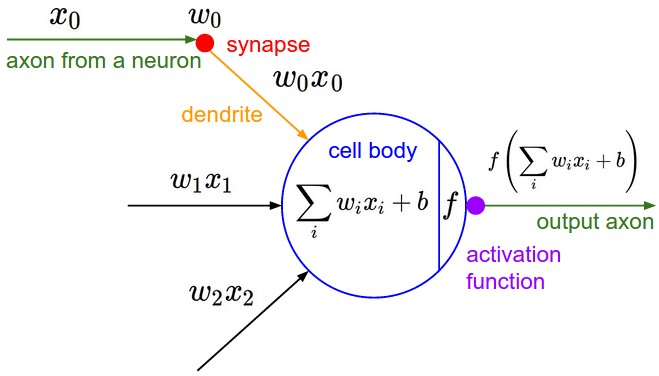
\includegraphics[scale = 0.35]{neuron_model.jpeg}
    \end{center}
  
    \bigskip 
  
  \begin{itemize}
    \setlength\itemsep{1em}
    \item[] \large \emph{Modello matematico di un neurone}
  \end{itemize}       
\end{frame} 


\begin{frame}{Reti Neurali}
    \framesubtitle{Funzionamento Neurone}
    \begin{itemize} [<+->]
        \setlength\itemsep{2em}
        \item \large Attraverso un meccanismo di eccitazione ed inibizione i pesi sinaptici controllano quanto un neurone venga influenzato dagli altri
       \item \large I segnali pesati dalle differenti sinapsi vengono trasportati dai dendriti all'interno del neurone e sommati tra loro
       \item \large Se la somma supera una certa soglia, il neurone \emph{spara} un segnale lungo l'assone 
       \item \large La \emph{frequenza di sparo} del neurone viene modellata con una funzione di attivazione $f$       
    \end{itemize}
\end{frame}


\begin{frame}{Reti Neurali}
    \framesubtitle{Funzioni di Attivazione}
    \begin{block}{Definizione} 
        \large Una \emph{funzione di attivazione} è una funzione matematica non lineare usata per calcolare l'output di un neurone. Riceve come input la somma pesata dei segnali in ingresso al neurone
    \end{block}\pause
    
    \begin{itemize} [<+->]
        \setlength\itemsep{2em}
        \item \emph{\large Sigmoide}
        \item \emph{\large Tangente Iperbolica}
        \item \emph{\large Softplus}
    \end{itemize}
\end{frame}

\begin{frame}{Reti Neurali}
    \framesubtitle{Sigmoide}
    \begin{block}{Definizione} 
        \large La \emph{Sigmoide} $\sigma: \mathbb{R} \rightarrow [0, 1]$ è definita come $\sigma(x) = \frac{1}{(1 + e^{-x})}$ 
    \end{block}\pause
    
    \begin{itemize} [<+->]
        \setlength\itemsep{2em}
        \item \large Per elevati valori negativi di input la sigmoide restituisce 0: il neurone non spara affatto
        \item \large Per elevati valori positivi di input la sigmoide restituisce 1: il neurone satura e spara con una frequenza di sparo pari a 1
        \item \large La sua derivata è uguale a $\sigma^{\prime}(x) = 1 - \sigma(x)$
    \end{itemize}
\end{frame}

\begin{frame}{Reti Neurali}
    \framesubtitle{Sigmoide}
    
    \begin{center}
      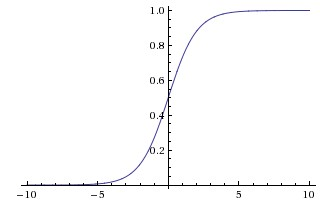
\includegraphics[scale = 0.6]{sigmoid.jpeg}
    \end{center}
  
    \bigskip 
  
  \begin{itemize}
    \setlength\itemsep{1em}
    \item[] \large \emph{Rappresentazione grafica Sigmoide}
  \end{itemize}       
\end{frame} 



\begin{frame}{Reti Neurali}
    \framesubtitle{Tangente Iperbolica}
    \begin{block}{Definizione} 
        \large La \emph{Tangente Iperbolica} $\tanh: \mathbb{R} \rightarrow [-1, 1]$ è definita come $\tanh(x) = 2\sigma(2x) - 1$ 
    \end{block}\pause
    
    \begin{itemize} [<+->]
        \setlength\itemsep{2em}
        \item \large La tangente iperbolica è una sigmoide scalata 
        \item \large La sua derivata è uguale a $\tanh^{\prime}(x) = 1 - \tanh^{2}(x)$
    \end{itemize}
\end{frame}

\begin{frame}{Reti Neurali}
    \framesubtitle{Tangente Iperbolica}
    
    \begin{center}
      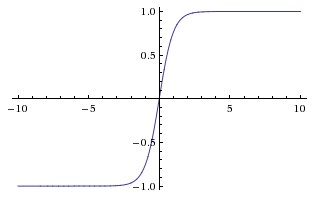
\includegraphics[scale = 0.6]{tanh.jpeg}
    \end{center}
  
    \bigskip 
  
  \begin{itemize}
    \setlength\itemsep{1em}
    \item[] \large \emph{Rappresentazione grafica Tangente Iperbolica}
  \end{itemize}       
\end{frame} 

\begin{frame}{Reti Neurali}
    \framesubtitle{Softplus}
    \begin{block}{Definizione} 
        \large La \emph{Softplus} $s: \mathbb{R} \rightarrow [0, +\infty]$ è definita come $s(x) = \log(1 + e^x)$ 
    \end{block}\pause
    
    \begin{itemize} [<+->]
        \setlength\itemsep{2em}
        \item \large La softplus è un approssimazione della \emph{Rectifier Linear Unit (ReLU)}
        \item \large Viene usata per sostituire la ReLU che presenta un punto di discontinuità in 0
        \item \large La sua derivata è uguale a $s^{\prime}(x) = \frac{1}{(1 + e^{-x})}$
    \end{itemize}
\end{frame}

\begin{frame}{Reti Neurali}
    \framesubtitle{Softplus}
    
    \begin{center}
      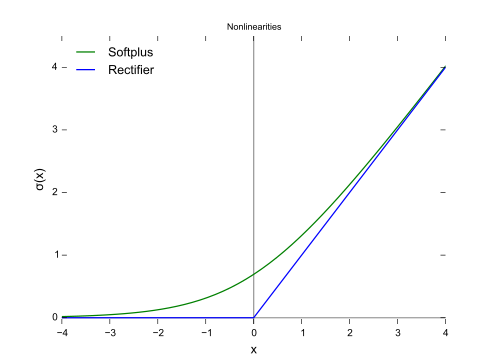
\includegraphics[scale = 0.45]{softplus_vs_rectifier.png}
    \end{center}
  
    \smallskip
  
  \begin{itemize}
    \setlength\itemsep{1em}
    \item[] \large \emph{Confronto grafico tra ReLU e Softplus}
  \end{itemize}       
\end{frame} 

\begin{frame}{Reti Neurali}
    \framesubtitle{Rete Neurale}
    
    \begin{block}{Definizione} 
        \large Una \emph{Rete Neurale} è composta da un insieme di neuroni connessi in un grafo aciclico. I neuroni sono organizzati come una serie di livelli (layer) distinti.
    \end{block}\pause
    \begin{itemize} [<+->]
        \setlength\itemsep{2em}
        \item \large Attraverso un meccanismo di eccitazione ed inibizione i pesi sinaptici controllano quanto un neurone sia influenzato dagli altri
    \end{itemize}
\end{frame}




\begin{frame}{Reti Neurali}
    \framesubtitle{Rete Neurale Convoluzionale}  
    Una \emph{Rete Neurale Convoluzionale} si differenzia da una più classica in quanto assume che l'input della rete sia un'immagine
\end{frame}   

\begin{frame}[c]
  \centering
  \bigskip \bigskip    
  \Huge Implementazione della Rete
\end{frame}

\begin{frame}[c]
  \centering
  \bigskip \bigskip    
  \Huge Analisi dei Risultati
\end{frame}


\end{document}
